\chapter{Réalisations techniques}
Comme énoncé dans la première partie de ce mémoire, nus allons concentrer notre travail sur la sécurisation des 
développements applicatifs jusqu'à leur déploiement. Nous aborderons donc des sujets tel que la création de deux 
procédures de sécurité, l'outillage des équipes ainsi que la réalisation de diverses évaluations de sécurité.

\section{Une première approche du DevSecOps}
Rapidement évoqué dans l'état de l'art, l'équipe de \ac{SSI} a entamée ,dès le quatrième semestre de 2018, un premier 
travail d'intégration de sécurité informatique dans les développements au travers de la mise en place d'un processus 
\emph{Security By Design}.

Ce processus, centré en son cœur sur l'accompagnement de \emph{Security Champions}\footnote{Un 
\emph{Security Champion} est un ambassadeur de la \ac{SSI} dans les équipes projets.}, vise à faciliter le questionnement
et  les réflexions sur les sujets de \ac{SSI} dans les équipes projets. Représentés par des responsables produit, des 
développeurs ou opérationnels, ils favorisent les échanges entre les équipes projets et l'équipe de \ac{SSI} en servant 
de réels points de liaisons pour ces dernières.

Grâce au travail des \emph{Security Champions}, le nombre de demande d'audit technique et de conseils d'architecture
a progressivement augmenté tout au long de l'année 2019. L'équipe s'est donc retrouvé à réaliser plusieurs audits par 
mois sur l'année 2019 là où elle n'en réalisait qu'un tous les deux mois en moyenne en 2018. J'ai par ailleurs eu le 
plaisir de m'occuper d'une majorité de ces qualifications sécurité.

C'est d'ailleurs sur cette même période qu'un projet de personnalisations des règles du \ac{SAST} (SonarQube) exploité 
par JCDecaux a été lancé. Ces personnalisations, réalisées en deux temps, visaient à créer plusieurs profils d'analyse 
pour chaque langage de programmation utilisé dans l'entreprise, tout en réduisant le bruit généré par des règles 
remontant trop de faux positif.

Grace à ces actions, portés tant auprès du Groupe qu'auprès de ses filiales, l'équipe de \ac{SSI} s'est rapproché un peu
plus de son objectif de sécurisation des applications développées en interne. Cette approche proactive et non plus 
réactive de sécurisation a notamment permis de réduire drastiquement le nombre d'applications rejetées à la suite d'une 
qualifications sécurité pré-déploiement en production.

Nous passions donc d'une méthodologie agile \emph{DevOps} à une méthodologie \emph{DevSecOps}.

\newpage

\section{Les audits : quel processus pour quel résultat}
Depuis 2019, nous (l'équipe de \ac{SSI}) avons observé une nette augmentation du nombre de qualification sécurité réalisées
aux profits des projets de développement. Cette augmentation, bien que bénéfique à l'objet de l'équipe, a eu pour effet 
de mettre en évidence divers problèmes ans l'organisation et la réalisation de ces audits.
\newline Il nous arrivait encore à cette période de devoir intérrompre la publication de certaines applications n'étant 
pas qualifiées, faute de procédures explicites et partagées à toutes les équipes de JCDecaux. Nous avons donc commencer à 
travailler sur la question avec l'aide de quelques équipes de la \ac{DSI} France.

La première réalisation dans cette quête de structure à été la définition claire et précise des points de contrôle et 
des vulnérabilités recherchées sur les applications. Ces points de contrôle sont fortement inspirés par l'OWASP Top ten
\autocite{owasp_top10_2017} et sont formulés dans un tableur servant à faire leur suivi durant l'audit. Chacun est 
ensuite associé à plusieurs états (testé ou non, risque et application de correctifs) ainsi qu'un commentaire le cas 
échéant.

A cette liste de points de contrôle est ensuite adossé une revue du projet sur SonarQube (note \ac{SAST}) et de la 
classification des entrés remontées par l'outil. Cette étape nous permets de prendre la mesure de la qualité du code de 
l'application audité mais aussi du niveau d'attention apporté par l'équipe de développement à son application.
\newline Nous avons en effet constaté que les projets ayant le plus de vulnérabilité et erreur de code remonté par 
SonarQube étaient géré par des équipe ayant peu d'intérêt dans le contrôle qualité de leur code.
\newline Ce même type de revue est réalisé le niveau de vulnérabilité des conteneurs pour les applications concernées, 
mais nous reviendrons sur ce sujet plus tard.

Nous avons par la suite commencé à travailler sur la définition des livrables et des points abordés durant la réunion de
restitution. Il est important de noté que ces livrables se limitaient jusque là à une simple liste de vulnérabilités
ordonnées en fonction de leur criticité et sans démonstration ou explication du chemin d'attaque.
\newline  La mise en place d'une restitution appropriée et argumentée de l'audit à permis de déceler quelques 
méconnaissance dans plusieurs équipes (notamment vis-à-vis du framework IAM du groupe) et sert souvent de point de départ 
à l'accompagnement des équipes entament leurs migration vers le DevSecOps.

Voilà donc comment fonctionnait le processus d'audit applicatif entre 2019 et 2020. 
\newline Cependant, ce processus étant tacite et non formaliser (la culture de l'orale étant encore très fort chez 
JCDecaux), plusieurs départs et changements de postes l'ont mis à mal.

C'est pourquoi nous avons entrepris de formuler ce processus dans un langage commun (ici le \ac{BPMN}) afin de le partager
aux équipes impliquées dans celui-ci. Nous en avons profité pour intégrer quelques prérequis facilitant l'organisation 
de l'audit technique et la création de garde-fous.

\newpage

Le processus d'audit est donc représenté sous la forme de deux diagrammes : le premier décrivant le fonctionnement 
générale de l'audit et des différents échanges entre l'équipe de développement et l'équipe de \ac{SSI}; le second 
décrivant les actions techniques réalisées durant l'audit.

\begin{figure}[h]
    \centering
    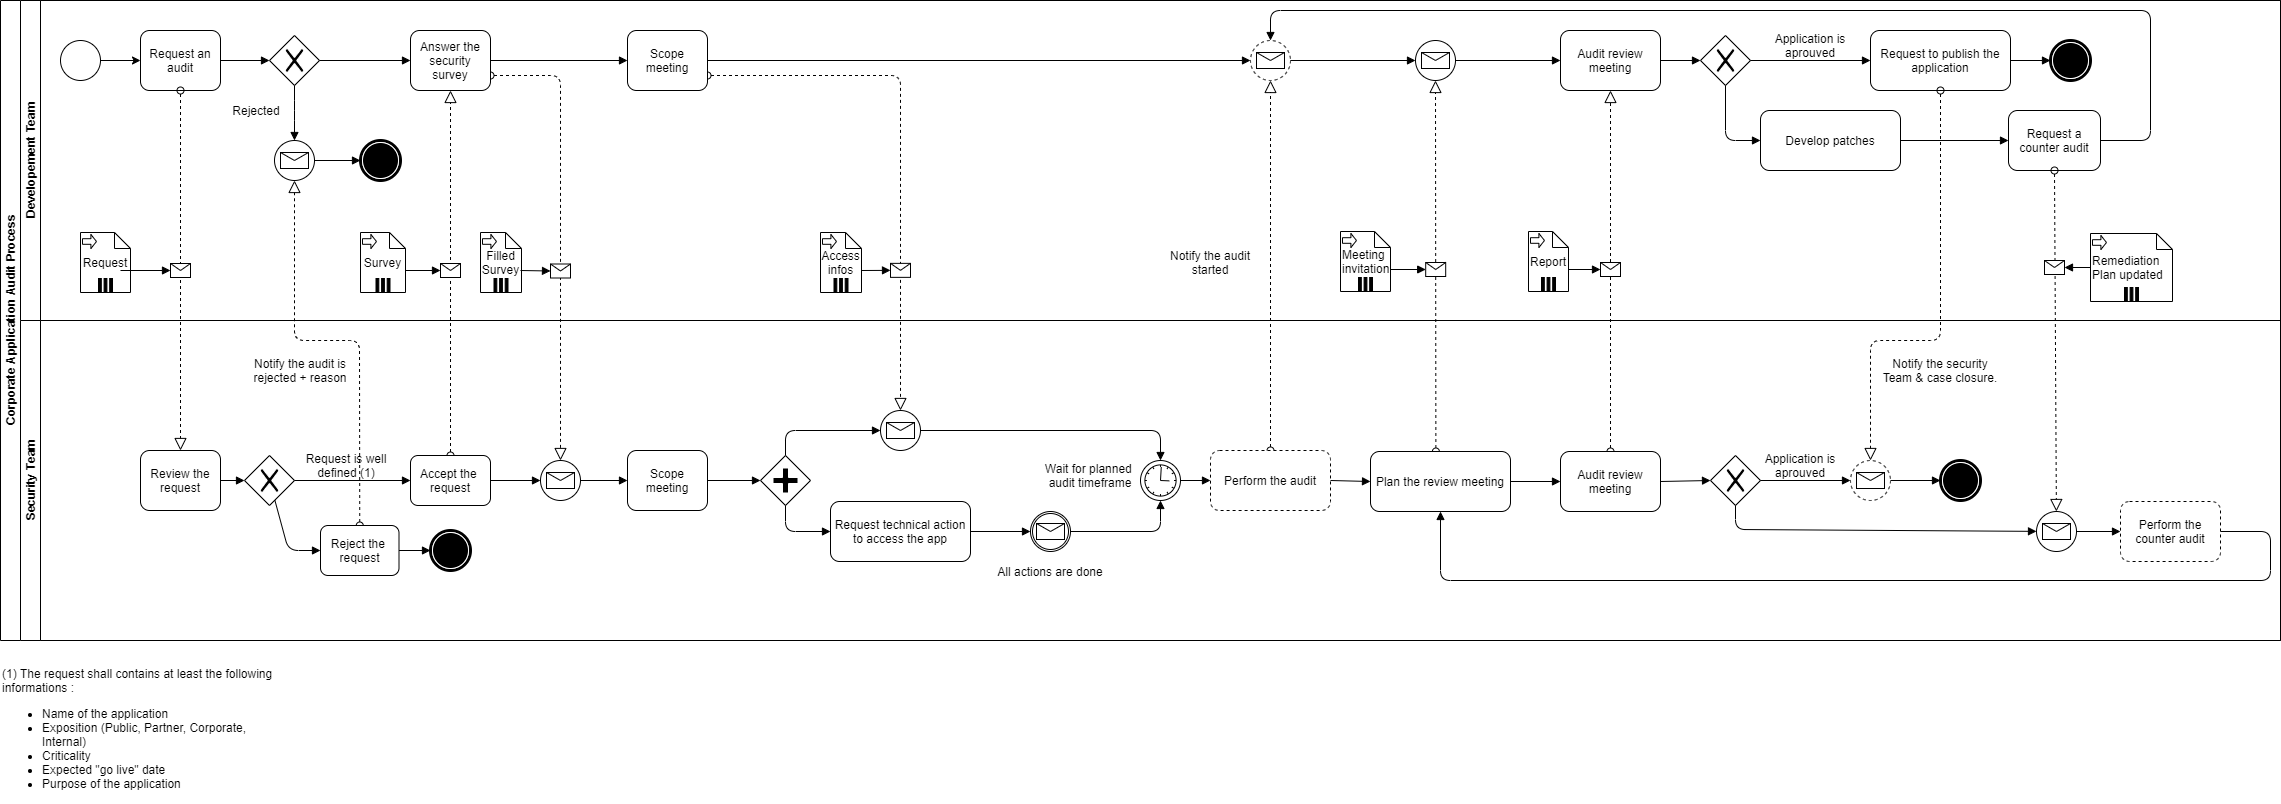
\includegraphics[width=\linewidth]{resources/img/process_audit.png}
    \caption{Processus de l'audit de sécurité d'une application}
\end{figure}

\begin{figure}[h]
    \centering
    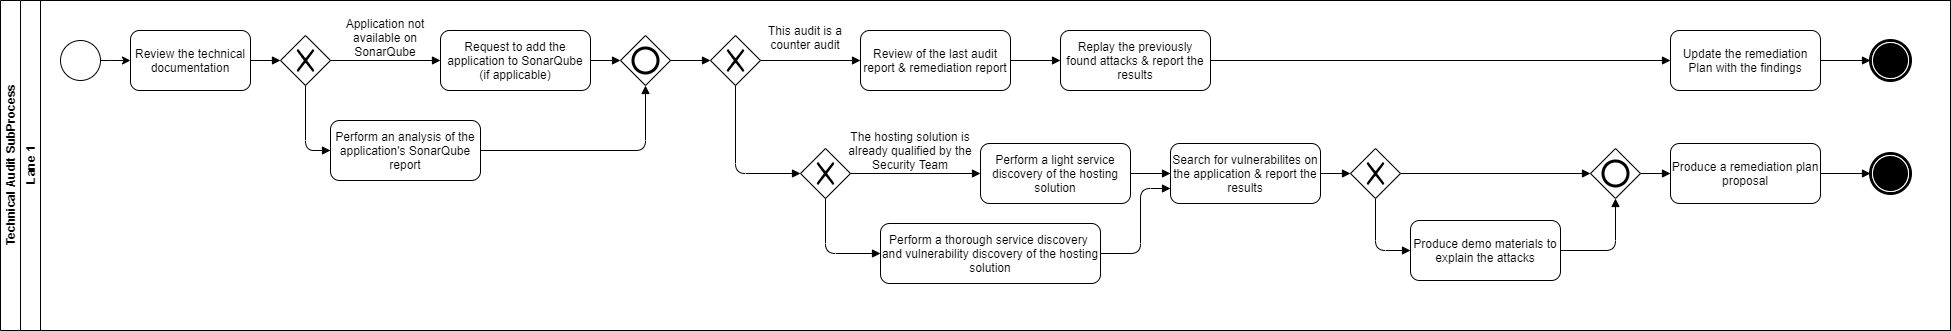
\includegraphics[width=\linewidth]{resources/img/technical_audit_subprocess.png}
    \caption{Processus fils de l'audit de sécurité d'une application : actions techniques}
\end{figure}
\begin{center}
    \colorbox{gray!15}{Ces deux diagrammes étant relativement complexes, vous les retrouverez en annexes}
\end{center}

Nous trouvons donc dans ce processus nouvellement formalisé l'ensemble des éléments précédemment évoqués avec l'ajout 
de quelques nouveautés nous permettant de mieux préparer l'audit. C'est ainsi qu'est intégré un questionnaire visant à
fournir à l'équipe de \ac{SSI} des informations supplémentaires sur la nature de l'application devant être audité ainsi 
que les éventuelles contraintes temporelles.

Ce processus étant en place dans sa version finale depuis Avril 2021, nous observons une amélioration progression des 
conditions d'organisation des audits techniques, notamment sur les éléments de contexte relatif aux applications devant 
être audités.
Il s'agissait en effet d'un certain point de friction de septembre 2020 suite au départ d'une de nos collaboratrices.

\newpage

\section{Inventaire et gestion de la sécurité des conteneurs}
Si la sécurité des applications est un sujet ayant fait l'office d'une certaine attention depuis ces trois dernières années
au sein du Groupe JCDecaux, la sécurité des conteneurs n'a pas eu cette chance faute de temps.
\newline Pour rappel, cette question n'a été abordée que brièvement lors des audits applicatifs jusqu'à la demande de 
mise en production de la plateforme \ac{K8S} et son audit par XMCO.

Le premier aspect de sécurité des conteneurs à adresser porte sur la création et le maintient d'un inventaire exhaustif
des \emph{Pods} en exécution sur les clusters et de leur état de vulnérabilité. S'il nous était possible d'extraire à la
main cet inventaire depuis un cluster \ac{K8S}, leur multiplication à la suite au cloisonnement de 
l'infrastructure a rendu la chose bien plus compliquée. Il nous faut donc nous équiper en consequence.

\subsection{Recherche d'outils}
Nous avons commencé à recherche des outils capables de nous fournir les informations nécessaires au suivi opérationnel 
des vulnérabilités des \emph{Pods} en fonctionnement. 

Cette recherche avait pour contraintes les éléments suivants :
\begin{itemize}
    \item Fonctionnement multi-cluster
    \item WebApplication pour la remontée des informations
    \item Mise à jours de l'inventaire automatique et journalière
    \item Export de rapport managériale
\end{itemize}

Quatre solutions ont correspondaient donc à notre besoin :
\begin{itemize}
    \item Le projet klustair (www.klustair.com)
    \item Le service de sécurité Kubernetes d'Aqua (www.aquasec.com)
    \item Le service de sécurité Kubernetes d'Alcide (www.alcide.io)
    \item Le service de scanner de vulnérabilité de Snyk (www.snyk.io)
\end{itemize}

Après une rapide analyse de ces solutions (voir tableau \ref{tab:sectoolscompkub}), nous constatons que si la solution 
\emph{Klustair} semblait correspondre au besoin, des fonctionnalités importantes sont manquantes. Notre choix devra donc
s'orienter vers les solutions commerciales.

Cependant, compte tenu de la crise du COVID-19 et du verrouillage des budgets nous ne pouvons plus lancer de projet à 
plus de 5 000€ dans l'accord du \ac{DAF}. Or, dans le cas des trois solutions restantes, la facture s'élèverait à minima
à \linebreak 25 000€ annuel.

Nous nous trouvons donc avec un dilemme : soit intégrer une solution peu sécurisée et remplissant une portion de nos 
besoin, soit entamer une négociation avec la direction afin de débloquer des budget et plus que probablement se voir 
refuser la proposition.
\newpage 

\begin{table}[h]
    \begin{center}
            \begin{tabular}{p{5cm}|llll}
                                                                & \textbf{Klustair} & \textbf{Aqua}              & \textbf{Alcide} & \textbf{Snyk}              \\
                \toprule
                \textbf{Coût license}                            & OpenSource        & \textgreater 2 000€ / mois & Inconnu         & \textgreater 3 000€ / mois \\
                \hline
                \textbf{Fonctionnement}                          & Auto-hébergé      & SaaS                       & SaaS            & SaaS                       \\
                \hline
                \textbf{Authentification}                        & Non               & Oui                        & Oui             & Oui                        \\
                \hline
                \textbf{Intégration registre Cloud}              & Oui               & Oui                        & Oui             & Oui                        \\
                \hline
                \textbf{Inventaire de Pods en fonctionnement}    & Oui               & Oui                        & Oui             & Oui                        \\
                \hline
                \textbf{Scanner de vulnérabilité}                & Oui               & Oui                        & Oui             & Oui                        \\
                \hline
                \textbf{Scanner de configuration / secrets}      & Possible          & Oui                        & Oui             & Oui                        \\
                \hline
                \textbf{Analyse de l'environnement d'execution}  & Non               & Oui                        & Oui             & Oui                        \\
                \hline
                \textbf{Export de rapport}                       & Non               & Non                        & Oui             & Oui                        \\
                \hline
                \textbf{Fréquence de mise à jour}                & Journalière       & Par heure                  & Par heure       & Par heure                 
            \end{tabular}
            \caption{Comparaison des produits de sécurité pour Kubernetes}
            \label{tab:sectoolscompkub}
    \end{center}
\end{table}

La solution à ce problème arrive cependant lorsque en Avril 2021 notre fournisseur de scanner de vulnérabilité 
d'infrastructure annonce l'intégration de fonctionnalités dédier à Kubernetes dans InsightVM, la solution déjà utilisée 
par l'équipe \ac{SSI}.

\subsection{Gestion de la sécurité des clusters avec InsightVM}
Après une rapide évaluation de faisabilité et experimentation des fonctionnalités nouvellement intégrées, nous prenons 
contact avec l'éditeur pour obtenir quelques informations supplémentaires sur les recommandations d'implémentations et 
la tarification des fonctionnalités. Aspect intéressant dans notre situation : seul le nombre d'agent de collecte déployé
est comptabilisé dans le nombre d'IP associé à la licence, le reste des fonctionnalités étant intégrées à celle souscrite
par JCDecaux.
\linebreak Cet entretien permet de confirmer le mode de fonctionnement l'agent de collecte, ainsi que des actions qu'il 
effectue sur le cluster. Le foncitonnement de l'agent et son intégration sur nos clusters est par ailleurs décrit dans 
un diagramme ci-après (voir diagramme \ref{figure:k8sscannerarchi}).

Suite à cet entretien, nous effectuons quelques ajustements sur la configuration de l'agent et le déployons
sur l'ensemble des clusters \ac{npr}. Ce déploiement sur six clusters distincts vis à évaluer l'exploitabilité de la 
plateforme Cloud Security\footnote{Plateforme SaaS de Rapid7 InsighVM dans laquelle est remonté l'ensemble des 
informations relatives aux registres de conteneur et clusters Kuberntes.} et des informations collectées. 

Lorsque nous analysons les données remontées sur la plateforme, nous constatons quelques erreurs et bugs dans le 
fonctionnement de la plateforme. Nous remontons donc ces points au support de l'éditeur et profitons de l'occasion
pour demander l'ajout de plusieurs évolutions pour la plateforme.
\newline Ces évolutions sont maintenant intégrées dans la feuille de route de l'éditeur. Elle devraient être intégrées 
dans la plateforme Cloud Security d'ici le troisième trimestre de 2021.

\begin{figure}[h]
    \centering
    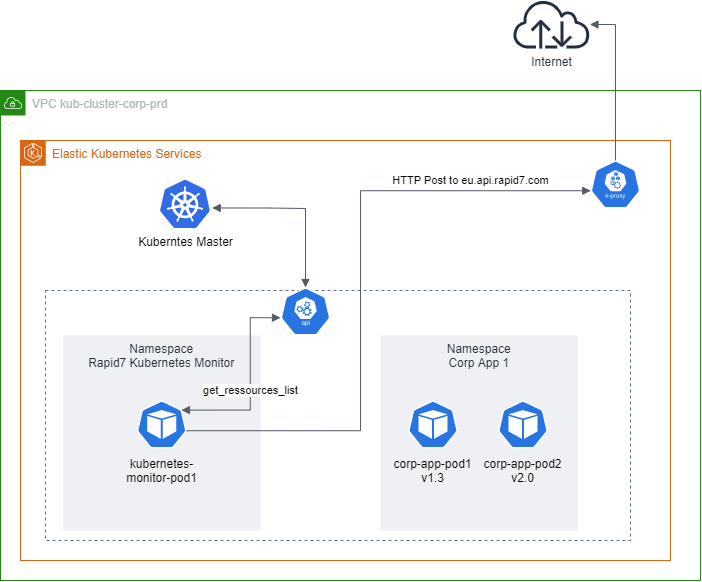
\includegraphics[width=\linewidth]{resources/img/k8s_scanner_archi.png}
    \caption{Schéma de déploiement de kubernetes-monitor sur un cluster Kubernetes}
    \label{figure:k8sscannerarchi}
\end{figure}

\subsection{Première revue de vulnérabilité des conteneurs}

Grâce l'intégration de l'inventaire des clusters Kubernetes sur notre plateforme de gestion opérationnel des vulnérabilités,
nous avons pu réaliser une première revue des images de conteneurs en fonctionnement sur les clusters de \ac{npr}.

Le premier constat que nous pouvons faire est plutôt positif : sur les 183 pod en cours d'exécution sur les clusters 
\ac{K8S}, seul 16 d'entre eux sont issues du registre DockerHub et n'ont donc pas été scanné par Rapid7.
\newline Ces \emph{pods} sont tous localisés dans l'espace de nom \emph{kube-system} et ne peuvent être intégrés sur notre
registre miroirs \ac{AWS} \ac{ECR}.

Cependant, on constate un nombre relativement haut de vulnérabilité (60 en moyenne) pour des conteneurs dont seul les 
paquets sont analysés. De plus, une majorité de ces conteneurs sont basés sur un système d'exploitation Centos 7,
système d'exploitation dont la date de fin de support est incertaine avec la migration de RedHat vers Centos Stream.

